%AXIOMATIC MODEL DEMYSTIFIED----------------------------------------------

\documentclass[10pt]{article}
\usepackage[utf8]{inputenc}
\usepackage{amsmath}
\usepackage{amssymb}
\usepackage[a4paper,margin=1in,footskip=0.25in]{geometry}
\usepackage[dvipsnames]{xcolor}
\usepackage{graphicx}
\usepackage{tikz}
\usepackage{amsthm}
\usepackage{float}
\usepackage{centernot}
\usepackage{tasks}

\title{ECMAScript Axiomatic Memory Consistency Model}
\author{Akshay Gopalakrishnan}
\date{November 2019}

\begin{document}

\maketitle


%Short form to use stack_relative
\newcommand{\stck}{\stackrel{\longrightarrow}}

%A different version of the above 
\newcommand{\stckdet}[1]{\stackrel{{#1}}}

%We write a lot of relations between two events using the orderings, so a short form to use that
\newcommand{\reln}[3]{#1\stck{_{#2}}#3}

%We use a more detailed version of the above relation to indicate direct / indirect relations 

\newcommand{\reldet}[4]{#1\stckdet{_{#2}}{{\stck{_{#3}}}}#4}

%We also will introduce a short form to write an event belongs to some set
\newcommand{\event}[2]{#1\!\in\!#2}

%To make events and their type more close to each other
\newcommand{\typ}[1]{\textit{#1}}
\newcommand{\et}[2]{#1\!:\!\typ{#2}}

%Short form to write color text
\newcommand{\critic}[2]{\textcolor{#1}{\footnotesize #2}}

%Some preliminary latex commands to format writing theorems 

\newtheorem{lemma}{Lemma}

\newtheorem{theorem}{Theorem}[lemma]

\newtheorem{corollary}{Corollary}[theorem]

\newtheorem{definition}{Definition}

%COMMENT FOR NOW AS IT IS NOT OUR PRIORITY 
%
\section{Introduction}
    Instruction reordering is a common transformation done by the compiler/hardware, which is essential to optimizations such as instruction scheduling, loop invariant removal, partial redundancy elimination, etc. 
    However, whether we can do such reordering freely given a concurrent program using relaxed memory accesses is a bit unclear. 
     
    \paragraph{Simple reordering is not straightforward under shared memory semantics}
    The main reason is that memory accesses here, do not just perform the desired operation (i.e Read / Write) but also imply certain visibility guarantees across all the other threads.  
    In our observation, we find that, the relaxed memory model of ECMAScript prescribe semantics for visibility using the $\stck{_{hb}}$ relations. 
    
    \paragraph{Some Examples}
        We show a couple of examples to showcase why reordering may not be that straightforward. 
        Consider the first example in Figure~\ref{reord:example1(a)} below of a Candidate before and after reordering two events.
        The original candidate is to the left and that on the right is after reordering the two reads of $T2$.
        The observable behavior in question is written in the middle(orange box). 
        \begin{figure}[H]
            \centering
            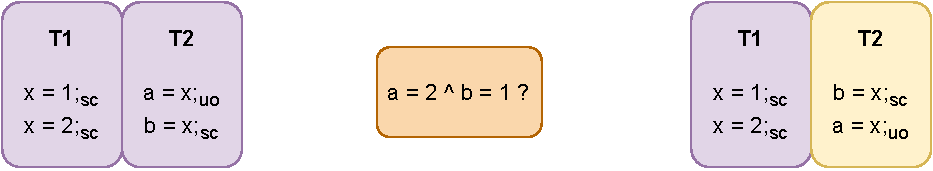
\includegraphics[scale=0.7]{5.InstructionReordering/0.Intro/ReorderingExample1(a).pdf}
            \caption{First example for reordering in candidates of the original program and its reordered counterpart.}
            \label{reord:example1(a)} 
        \end{figure}
        
        Figure~\ref{reord:example1(b)} has two sets of relations. 
        The first justifies the outcome for the reordered Candidate. 
        While the second justifies for the original Candidate. 
        Notice that in the first set of relations, we can infer that one may have a read memory ordered before a write that it reads from. 
        This is quite counter intuitive to understand at first. 
        But strictly from the semantics of the model, this justification to the observable behavior is completely valid\footnotemark. 
        \begin{figure}[H]
            \centering
            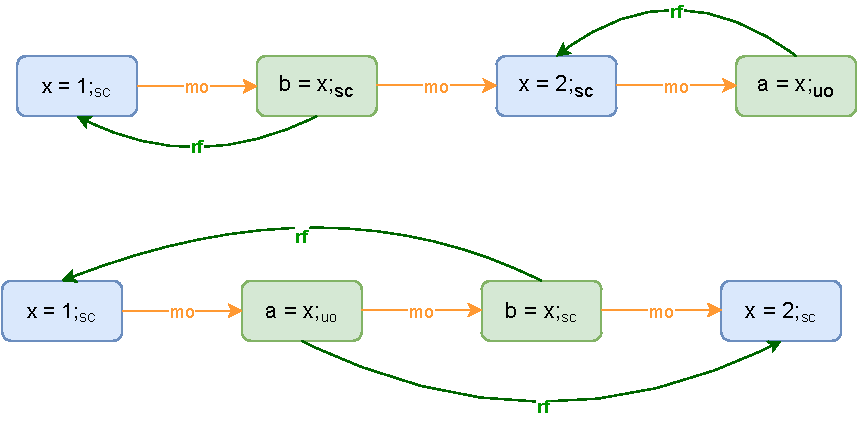
\includegraphics[scale=0.7]{5.InstructionReordering/0.Intro/ReorderingExample1(b).pdf}
            \caption{The set of partial order relations justifying the observable behavior in question for both the candidates in Figure~\ref{reord:example1(a)}.} 
            \label{reord:example1(b)}
        \end{figure}

        \footnotetext{In practice, this can be due to read speculation at the hardware level.}
        
        Consider another example in Figure~\ref{reord:example2(a)}.
        The figure on the left is the original candidate and that on the right is after reordering the two events of $T1$.
        The observable behavior in question is written in the middle(orange box). 
        \begin{figure}[H]
            \centering
            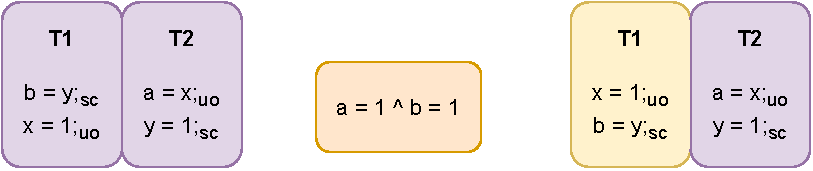
\includegraphics[scale=0.7]{5.InstructionReordering/0.Intro/ReorderingExample2(a).pdf}
            \caption{Second example for reordering with candidates of the original program and its reordered counterpart.} 
            \label{reord:example2(a)}
        \end{figure}
   
        Figure~\ref{reord:example2(b)} has two sets of relations. 
        The first justifies that such an outcome is not possible for the original program candidate due to Axiom \ref{CoRe}. 
        While the second justifies that this outcome is possible for the reordered program.
        Note that we cannot infer in the reordered candidate the set of relations for any candidate execution to have $\reln{a=x;_{uo}}{hb}{x=1;_{uo}}$. 
        \begin{figure}[H]
            \centering
            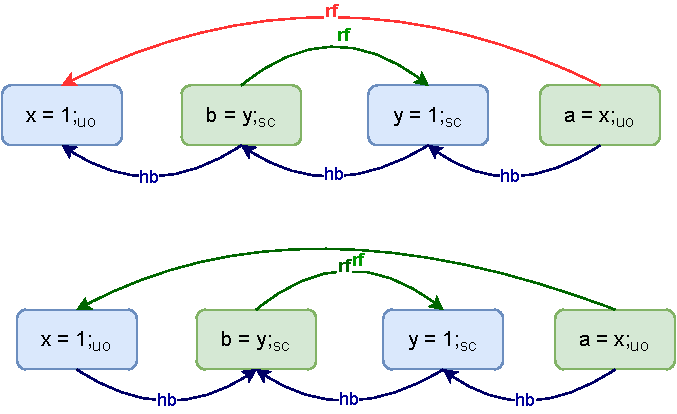
\includegraphics[scale=0.7]{5.InstructionReordering/0.Intro/ReorderingExample2(b).pdf}
            \caption{The set of partial order relations justifying the observable behavior in question for both the candidates in Figure~\ref{reord:example2(a)}.} 
            \label{reord:example2(b)}
        \end{figure}

        The above two examples show that we have to be careful while reordering two events in the same thread. 
        By example analysis, for each observable behavior, one must check all possible candidate executions and assert whether such an observable is possible or not. 
        This method of checking validity of reordering will scale exponentially as the program size increases. 
        It may also be the case that the compiler may not have information on which exact events would be executed in other threads to assert such reordering is valid. 

    
    
    
    
    


%The ECMAScript Memory Model

%AGENTS----------------------------------------------------------------------------------------------------------------------------------------  
\section{Agents, Events and their Types}

    \subsection{Agents}
        A concurrent program involves different threads/processes running concurrently. Agents are analogous to different threads/processes. 
        
        \critic{red}{Agents actually have more meaning than what we refer to here. However, in terms of reasoning just with memory consistency rules, we are safely abstracting them to just mean threads/processes.}

        %Agent Clusters
        \paragraph{Agent Cluster}
        Collection of agents concurrently communicating with each other (directly/ indirectly) form an agent cluster.  There can be multiple agent clusters. However, an agent can only belong to one agent cluster.

        \critic{red}{Please look back at what Conrad had said to about agent clusters.}
        
        %Perhaps give an example here later

        \critic{blue}{Note that for the purpose of reasoning with optimizations given the memory model, we stick to assuming that just one agent cluster exists. We also assume that agents in the cluster communicate only through one common shared memory segment.}

        \critic{purple}{Could elaborate the role when different shared array buffers are used to communicate accross agents belonging to different clusters. However, this is something that is not primary to our purpose of investigation, but would be essential as a whole from a practical standpoint to enforce correct concurrent programming.}
        
        %Agent Event Set
        \paragraph{Agent Event List $(ael)$}
        Every agent is mapped to a list of events. Operationally (when a program actually runs),  these events are appended to the list during evaluation. We define $ael$ is a mapping of each agent to a list of events.
        
            \[ael(a) = [e_1, e_2, ... e_k ] \]
        
        \critic{blue}{The standard refers this to be an Event List, but we find it a bit misleading as it does not signify a list for each agent. Hence we name it as Agent Event List}

        

            



%Events------------------------------------------------------------------
    \subsection{Events}
        
        An evaluation of an operation results in a set of events that are evaluated. An event is either an operation that involves (shared) memory access or that constrains the order of execution of multiple events. The latter are called \textit{Synchronize Events}

        \critic{blue}{Synchronizing events are analogous to $lock$ and $unlock$ events that allow exclusive access to critical sections of memory.}  

%Events----------------------------------------------------------------------------------------------------------------------------------
    
    %Useful command syntax
    \newcommand{\rmw}{\textit{rmw}\,}
    \newcommand{\set}[1]{\textbf{\textit{#1}}}

%Events------------------------------------------------------------------
    \subsection{Events}
    Agent execution is modelled in terms of events. 
    An event, in our context, is either an operation that involves (shared) Read/Write memory access or Synchronize events that constrains the order of execution of multiple events. 
    We define \set{E} as the set of events involved in an agent cluster. 
    We refer to \set{SM}, \set{R}, \set{W}, \set{S} as sets of Shared Memory, Read, Write and Synchronize events respectively. Read-Modify-Write events belong to both \set{R} and \set{W}. 
       
        \subsubsection{Range ($\Re$)}
            Each of the \textit{shared memory events} are associated with a contiguous range of memory on which it operates. $\Re$ is a function that maps a shared memory event to the range of memory indices it operates on which we represent as a starting index $i$ and a size $s$. As an example, the range of event $e$ would be like: 
                    
                    \[\Re(w) = (i, s) \]
           
            %\critic{red}{The range as per the ECMAScript standard denotes only the set of contiguous byte indices. The starting byte index is kept separate. We find this to be unnecessary. Hence we define range to have starting index and size.}
           
            We define two binary operators $\cap_\Re$ and $\cup_\Re$ to give the intersection and union respectively of the set of the byte indices, in order to describe disjoint, overlapping and equal ranges.  
            
%Types of Events Based on Order--------------------------------------------------------------------------------------------------------------------
    \subsubsection{Types of events based on Order} 
        There are 3 types (or access modes) which play a role in the sequence in which event actions are visible to different agents
        \begin{enumerate}
            \item \textbf{Sequentially Consistent ($sc$)} - Events of this type are $atomic$ in nature. There is a strict global total ordering of such events which is agreed upon by all agents in the agent cluster. 
            
            \item \textbf{Unordered ($uo$)} - Events of this type are considered non-atomic and can occur in different orders for each agent.
            
            \item \textbf{Initialize ($init$)} - Events of this type are used to initialize the values in memory ordered before events in an agent cluster.
        \end{enumerate}
        
        All events of type \textit{init} are writes and all read modify write events are of type \textit{sc}.
        We represent the type of events in the memory consistency rules in the format ``$\textit{event} : \textit{type}$''. 
        When representing events in a figure, the type would be represented as a subscript: $\textit{event}_\textit{type}$.
   
%Tearing factor of events
    \subsubsection{Tearing (or not)}
        Additionally, each shared-memory event is also associated with a tearing factor. 
        Events that tear are non-aligned accesses requiring more than one memory access. Events that are tear-free are aligned and should appear to be serviced in one memory access. The implication of tearing is better understood with the consistency rule that will later be shown.

%Relation among events----------------------------------------------------------------------------------------------------------------------------
    \subsection{Relation among events}
        We now describe a set of binary relations between events. These relations help us describe the consistency rules.
        
        \subsubsection{Read-Write event relations}
        There are two basic relations that assist us in reasoning about read and write events.
        
            %Read bytes from relation 
            \paragraph{Read-Bytes-From $(\stck{_{rbf}})$}
            
            This relation maps every read event to a list of tuples consisting of write event and their corresponding byte index that is read. For instance, consider a read event $r[i...(i+3)]$ and corresponding write events $w_1[i...(i+3)]$, $w_2[i...(i+4)]$. One possible $\stck{_\textit{rbf}}$ relation could be represented as  
                \begin{align*}
                    \reln{e}{\textit{rbf}}{\{(d1, i), (d2, i\!+\!1), (d2, i\!+\!2)\}}     
                \end{align*}   
            or having individual binary relation with each write-index pair as 
            \begin{align*}
                \reln{e}{rbf}{(d1, i)},\ \reln{e}{rbf}{(d2, i\!+\!1)}  \text{ and } \reln{e}{rbf}{(d2, i\!+\!2)}.
            \end{align*}
            
            %Reads from relation
            \paragraph{Reads-From $(\stck{_{rf}})$}
            
            This relation, is similar to the above relation, except that the byte index details are not involved in the composite list. So for the above example, the \textit{rf} relation would be represented either as   
                $\reln{e}{rf}{(d1, d2)}$
            or individual binary read-write relation as 
                $\reln{e}{rf}{d1}$ and $\reln{e}{rf}{d2}$.
            Figure below is an example of a program with its outcome (read values) shown in terms of reads-from relations. 
            \begin{figure}[H]
                \centering
                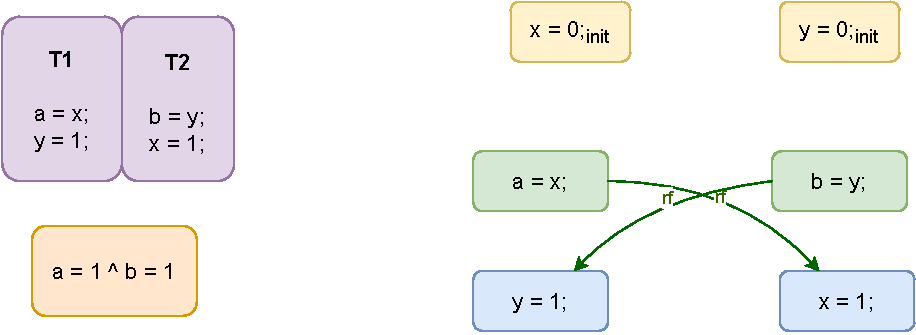
\includegraphics[scale=0.7]{ECMAScriptMemoryModel/ReadsFrom.pdf}
                \caption{An example to show the reads-from relations that are drawn for the example program between read and write events.}
                \label{read-from}
            \end{figure}
            
            %Agent sync with relation
        \subsubsection{Agent-Synchronizes With (\set{ASW})}
        
            It is a list for each agent that consist of ordered tuples of synchronize events. These tuples specify ordering constraints among agents at different points of execution. So such a list for an agent $k$ would be represented like:  
                \[ASW_k = \{ \langle s_1, s_2 \rangle, \langle s_3, s_4 \rangle ...\}\]
        
            For every pair in the list, the second event belongs to the parent agent and the first belongs to another agent it synchronized with\footnotemark.
                \[  
                    \forall{i,j>0},\ 
                    \langle s_1, s_2 \rangle \in ASW_j 
                    \Rightarrow{} 
                    s_2 \in ael(k)                        
                \]

            The figure below shows an example of this relation among two agents. 
            \begin{figure}[H]
                \centering
                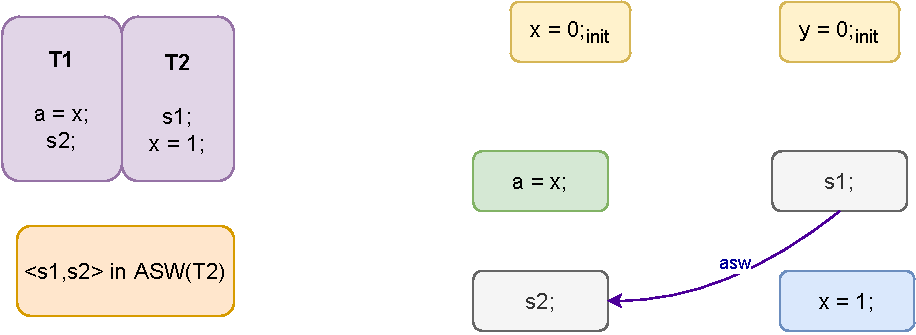
\includegraphics[scale=0.7]{ECMAScriptMemoryModel/AgentSyncWith.pdf}
                \caption{An example to show the reads-from relations that are drawn for the example program between read and write events.}
                \label{agent-sync-with}
            \end{figure}
        
        \footnotetext{This is analogous to the property that every unlock must be paired with a subsequent lock, which enforces the condition that a lock can be acquired only when it has been released.}

%Ordering Relation among Events----------------------------------------------------------------------------------------------------------------------       
        \section{Ordering Relations among Events}
        
        %Agent Order
        \paragraph{Agent Order ($\stck{_{ao}}$)}
            A total order among events belonging to the same agent event list. It is analogous to intra-thread ordering. For example, if two events $e$ and $d$ belong to the same agent event list , then either $\reln{e}{\textit{ao}}{d}$ or $\reln{d}{\textit{ao}}{e}$. 
            
            \critic{blue}{Note that the relations are only with respect to events belonging to the same agent. A collection of such relations together form the agent order. This is analogous to what we know as intra-thread sequential order. It is also the same as what \textbf{sequenced-before} is defined to be in C++.}

            \critic{purple}{Sequenced before maybe a bit weaker that agent order, as we saw in one of the papers. Basically, sequenced before precisely tells us which events can be reordered and which cannot, in contrast to agent order. I think it is similar to preserved program order in hardware, which is defined to capture dependancies resulting due to control flow in programs. Do check and see if these are the same. Discuss with Clark. }
        
        %Synchronize With Order
        \paragraph{Synchronize-With Order ($\stck{_{sw}} $)}
            Represents the synchronizations among different agents through relations between their events. It is a composition of two sets as below: 
            \begin{enumerate}
                \item All pairs belonging to $ASW$ of every agent belongs to this ordering relation. 
            
                        \[\forall{i, j > 0}, \ \langle e_i, e_j \rangle \in ASW \Rightarrow{} e_i \stck{_{sw}} e_j \]
            
                \item Specific reads-from pairs also belong to this ordering relation. 
            
                        \[(r \stck{_{rf}} w) \ \wedge \ \et{r}{sc} \ \wedge \ \et{w}{sc} \ \wedge \ (\Re(r)\!=\!\Re(w)) \ \Rightarrow{} \ (w \stck{_{sw}} r)\]
            
            \end{enumerate}
            
            \critic{blue} {Note that for the second condition, both ranges of events have to be equal. This however, does not mean that the read cannot read from multiple write events. (the read-from relation here is not functional.)}
            
        %Happens Before order 
        \paragraph{Happens Before Order ($\stck{_{hb}}$)}
            A transitive order on events, composed of the following:
            
            \begin{enumerate}
                \item Every agent-ordered relation is also a happens-before relation 
              
                    \[(e \stck{_{ao}} d) \ \Rightarrow{} \ (e \stck{_{hb}} d)\]
              
                \item Every synchronize-with relation is also a happens-before relation 
              
                    \[(e \stck{_{sw}} d) \ \Rightarrow{} \ (e \stck{_{hb}} d)\]
                     
                \item Initialize type of events happen before all shared memory events that have overlapping ranges with them. 
                
                    \[
                        \forall e,d \in SM \ \wedge \ 
                        \et{e}{init} \ \wedge \ 
                        (\Re(e) \cap \Re(d) \neq \phi)
                        \ \Rightarrow{} \ 
                        e \stck{_{hb}} d
                    \]
            \end{enumerate}
        
        \critic{red}{It is also important to note that those $\stck{_{hb}}$ relations that are formed due to Sequentially Consistent events (read-write), imply a more stronger visibility guarantee, in that all the threads observe the same global total order of such events. This however, is not expressed using this relation. Perhaps a better way to represent it may be required.}
        
        %Memory Order
        \paragraph{Memory Order ($\stck{_{mo}}$)}
            This order is a \textit{total order} on all events that respects happens-before order. 
                \[(e \stck{_{hb}} d) \Rightarrow{} (e \stck{_{mo}} d)\]
          

    \subsection{Preliminaries}
    Before we go about proving when reordering is valid, we would like to have two additional definitions which would prove useful.
    
    %Something we need to define for sake of proofs
    \begin{definition}{Consecutive pair of events (\emph{cons})}
        
        We define \emph{cons} as a function, which takes two events as input, and gives us a boolean indicating if they are consecutive pairs. Two events $e$ and $d$ are consecutive if they have an $\stck{_\textit{ao}}$ relation among them and are \emph{next to each other} in the same agent (thread), which can be defined formally as 
            \begin{align*}
                (
                e \stck{_\textit{ao}} d  \ \wedge \ 
                \nexists k \ \textit{s.t.} \ 
                e \stck{_\textit{ao}} k  \ \wedge \
                k \stck{_\textit{ao}} d 
                )
                \ \vee \
                (
                    d \stck{_\textit{ao}} e  \ \wedge \ 
                    \nexists k \ \textit{s.t.} \ 
                    d \stck{_\textit{ao}} k  \ \wedge \
                    k \stck{_\textit{ao}} e  
                )
            \end{align*}
    \end{definition}

    \begin{definition}{Direct happens-before relation (dir)}
        
        We define \emph{dir} to take an ordered pair of events $(e,d)$ such that $\reln{e}{hb}{d}$ and gives a boolean value to indicate whether this relation is \textit{direct}, i.e those relations that are not derived through transitive property of $\stck{_\textit{hb}}$.

        %Perhaps put a formal defintion here 
        
        We can infer certain relations/conditions that must hold using this function based on some information on events $e$ and $d$. 
        \begin{itemize}
            \item If $\et{e}{uo}$, then $dir(e,d) \ \Rightarrow \ cons(e,d)$
            \item If $\et{d}{uo}$, then $dir(e,d) \ \Rightarrow \ cons(e,d)$
            \item If $\et{e}{sc}\ \wedge\ e\!\in\!R$, then $dir(e,d) \ \Rightarrow \ cons(e,d)$
            \item If $\et{e}{sc}\ \wedge\ e\!\in\!W$, then $dir(e,d) \ \Rightarrow \ cons(e,d)\ \vee\ \reln{e}{sw}{d}$
            \item If $\et{d}{sc}\ \wedge\ d\!\in\!W$, then $dir(e,d) \ \Rightarrow \ cons(e,d)$
            \item If $\et{d}{sc}\ \wedge\ e\!\in\!R$, then $dir(e,d) \ \Rightarrow \ cons(e,d)\ \vee\ \reln{e}{sw}{d}$
        \end{itemize}
    \end{definition}


%Valid Execution Rules---------------------------------------------------------------------------------------------------------------------------------
    %MAKE SURE TO PLACE DEFINITONS ON PROGRAM, CANDIDATE, CANDIDATE EXECUTION and OBSERVABLE BEHAVIOURS        

    \subsection{Valid Execution Rules (the Axioms)}
        We now state the memory consistency rules. The rules are on \textit{Candidate Executions} which will place constraints on the possible \textit{Observable behaviors} that may result from it.
         
        %Coherent Reads   
        \subsubsection{Coherent Reads} 
        
            There are certain restrictions of what a read event cannot see in an execution based on $\stck{_\textit{hb}}$ relation with write events.
            
            Consider a read event $e$ and a write event $d$ having at least overlapping ranges:
            \begin{align*}
                \event{e}{R} \ \wedge \ 
                \event{d}{W} \ \wedge \
                (\Re(e) \cap_\Re \Re(d) \neq \phi).
            \end{align*}
            
            A read value cannot come from a write that has happened after it or if there is a write $g$ that happens between them, writing at the same memory.     
                \begin{gather*}
                    \reln{e}{hb}{d}\ \Rightarrow{}\ \neg \ \reln{e}{rf}{d}. \\
                    \reln{d}{hb}{e}
                    \ \wedge \ 
                    \reln{d}{hb}{g} \ \wedge \  \reln{g}{hb}{e}
                    \ \Rightarrow{} \
                    \forall x \in (\Re(d) \cap_\Re \Re(g) \cap_\Re \Re(e)), \ \neg \ \reln{e}{rbf}{(d,x)}.
                \end{gather*}
     
      \subsubsection{Tear-Free Reads} 
               If two tear free writes $d$ and $g$ and a tear free read $e$ all with equal ranges exist, then $e$ can read only from one of them
                \begin{align*}
                      \et{d}{tf}\ \wedge\ \et{g}{tf} \ \wedge \ \et{e}{tf} 
                        \ \wedge \ 
                        (\Re(d) \!=\! \Re(g) \!=\! \Re(e)) 
                        \ \Rightarrow{} \ 
                            ((\reln{e}{rf}{d}) 
                            \ \wedge \ 
                            (\neg \ \reln{e}{rf}{g})) 
                        \ \vee \  
                            ((\reln{e}{rf}{g}) 
                            \ \wedge \
                            (\neg \ \reln{e}{rf}{d})).
                \end{align*}
                    
        \subsubsection{Sequentially Consistent Atomics} 
            To specifically define how events that are sequentially consistent affects what values a read cannot see, we assume the following memory order among writes $d$ and $g$ and a read $e$ to be the premise for all the rules: 
                \begin{align*}
                    d \stck{_{mo}} g \stck{_{mo}} e.
                \end{align*}
            There are three separate rules that restrict reads-from relation between $d$ and $e$
                \begin{gather*}
                        \et{d}{sc}\ \wedge\ \et{g}{sc}\ \wedge\ \et{e}{sc} 
                        \ \wedge \ (\Re(d) \!=\! \Re(g) \!=\! \Re(e))
                        \ \Rightarrow{} \ 
                        \neg \ \reln{e}{rf}{d}.
                    \\    
                        \et{d}{sc}\ \wedge\ \et{g}{sc}  
                        \ \wedge \ (\Re(d) \!=\! \Re(g)) 
                        \ \wedge \ \reln{d}{hb}{e}
                        \ \wedge \ \reln{g}{hb}{e}
                        \ \Rightarrow{}\  
                        \neg \ \reln{e}{rf}{d}.
                    \\
                        \et{g}{sc}\ \wedge\ \et{e}{sc}  
                        \ \wedge \ (\Re(g) \!= \!\Re(e)) 
                        \ \wedge \ \reln{d}{hb}{g} 
                        \ \wedge \ \reln{d}{hb}{e}
                        \ \Rightarrow \ 
                        \neg \ \reln{e}{rf}{d}.
                \end{gather*}
  

%Races----------------------------------------------------------------------------------------------------------------------------------
        
    \section{Race}
        
        \paragraph{Race Condition $RC$} 
            We define \set{RC} as the set of all pairs of events that are in a race. Two events $e$ and $d$ are in a race condition when they are shared memory events:
            \begin{align*}
                (e \in SM)\ \wedge\ (d \in SM).
            \end{align*}
            having overlapping ranges, not having a $\stck{_\textit{hb}}$ relation with each other, and which are either two writes or the two events are involved in a $\stck{_\textit{rf}}$ relation with each other. This can be stated concisely as,
            \begin{align*}
                \neg \ (\reln{e}{hb}{d})\ \wedge\ \neg \ (\reln{d}{hb}{e}) 
                \ \wedge \ 
                (
                (\event{e,d}{W}\  \wedge\ (\Re(d) \cap_{\Re} \Re(e) \neq \phi)) 
                    \  \vee\ (d \stck{_\textit{rf}} e)\ \vee\ (e \stck{_\textit{rf}} d)
                ).
            \end{align*}
            
             \critic{blue}{Though we say it as write events, they also encompass read-modify-write events, as specified by the axiom above.}    
        
        \paragraph{Data Race $DR$} 
            We define \set{DR} as the set of all pairs of events that are in a data-race. Two events are in a data race when they are already in a race condition and when the two events are not both of type \textit{sc}, or they have overlapping ranges. This is concisely stated as:  
            \begin{align*}
                \event{e,d}{RC}  \ \wedge \ 
                ((\neg\et{e}{sc} \ \vee \ \neg\et{d}{sc}) \ \vee \ 
                (\Re(e) \cap_{\Re} \Re(d) \neq \Re(e) \cup_{\Re} \Re(d))) 
            \end{align*}
            
            \critic{red}{The definition for data race also implies that sequentially consistent events with overlapping ranges are also in a data race. This may be counter-intuitive in the sense that all agents observe the same order in which these events happen.}
        
        
        \paragraph{Data-Race-Free (DRF) Programs}
            An execution is considered data-race free if none of the above conditions for data-races occur among events. A program is data-race free if all its executions are data race free.          
            \textit{The memory model guarantees Sequential Consistency for all data-race free programs (SC-DRF).}
        

%Consistent Executions-------------------------------------------------------------------------------------------------------------------

   %Consistent Executions-------------------------------------------------------------------------------------------------------------------

   \subsection{Consistent Executions (Valid Observables)}
        A valid observable behaviour is when\footnotemark:
        \begin{enumerate}
           \item No $\stck{_\textit{rf}}$ relation violates the above memory consistency rules.
           \item $\stck{_\textit{hb}}$ is a strict partial order.
        \end{enumerate} 

        \textit{The memory model guarantees that every program must have at least one valid observable behaviour.}

        \footnotetext{There is also some conditions on host-specific events (which we mentioned is not of our main concern) and what is called a chosen read, which is nothing but the reads that the underlying hardware memory model allows. Since we are not concerned with the memory models of different hardware, this restriction on reads is not of our concern.}
    
    
\input{InstructionReordering/reordering_opt.tex}


\section{Introduction}
    Instruction reordering is a common transformation done by the compiler/hardware, which is essential to optimizations such as instruction scheduling, loop invariant removal, partial redundancy elimination, etc. 
    However, whether we can do such reordering freely given a concurrent program using relaxed memory accesses is a bit unclear. 
     
    \paragraph{Simple reordering is not straightforward under shared memory semantics}
    The main reason is that memory accesses here, do not just perform the desired operation (i.e Read / Write) but also imply certain visibility guarantees across all the other threads.  
    In our observation, we find that, the relaxed memory model of ECMAScript prescribe semantics for visibility using the $\stck{_{hb}}$ relations. 
    
    \paragraph{Some Examples}
        We show a couple of examples to showcase why reordering may not be that straightforward. 
        Consider the first example in Figure~\ref{reord:example1(a)} below of a Candidate before and after reordering two events.
        The original candidate is to the left and that on the right is after reordering the two reads of $T2$.
        The observable behavior in question is written in the middle(orange box). 
        \begin{figure}[H]
            \centering
            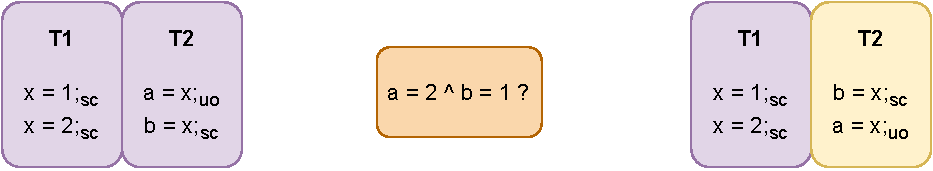
\includegraphics[scale=0.7]{5.InstructionReordering/0.Intro/ReorderingExample1(a).pdf}
            \caption{First example for reordering in candidates of the original program and its reordered counterpart.}
            \label{reord:example1(a)} 
        \end{figure}
        
        Figure~\ref{reord:example1(b)} has two sets of relations. 
        The first justifies the outcome for the reordered Candidate. 
        While the second justifies for the original Candidate. 
        Notice that in the first set of relations, we can infer that one may have a read memory ordered before a write that it reads from. 
        This is quite counter intuitive to understand at first. 
        But strictly from the semantics of the model, this justification to the observable behavior is completely valid\footnotemark. 
        \begin{figure}[H]
            \centering
            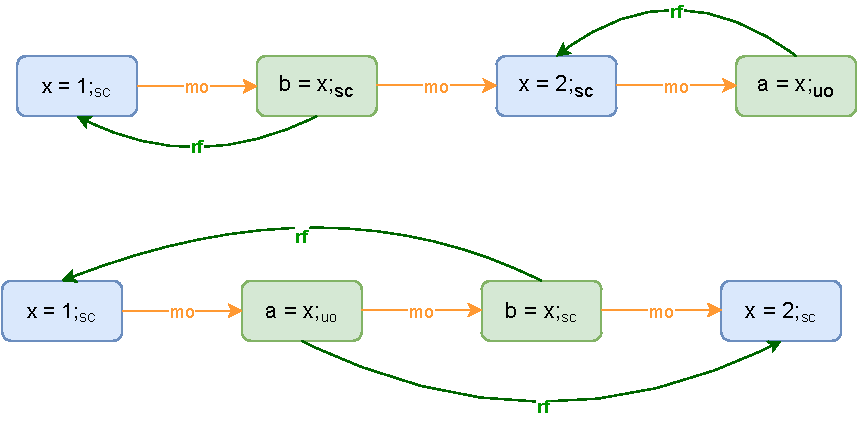
\includegraphics[scale=0.7]{5.InstructionReordering/0.Intro/ReorderingExample1(b).pdf}
            \caption{The set of partial order relations justifying the observable behavior in question for both the candidates in Figure~\ref{reord:example1(a)}.} 
            \label{reord:example1(b)}
        \end{figure}

        \footnotetext{In practice, this can be due to read speculation at the hardware level.}
        
        Consider another example in Figure~\ref{reord:example2(a)}.
        The figure on the left is the original candidate and that on the right is after reordering the two events of $T1$.
        The observable behavior in question is written in the middle(orange box). 
        \begin{figure}[H]
            \centering
            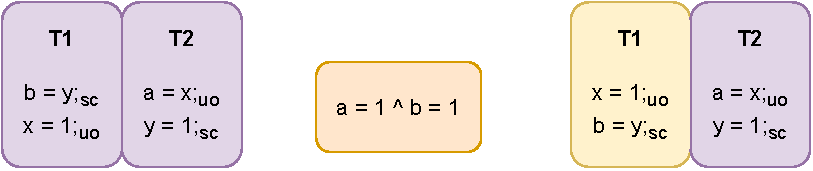
\includegraphics[scale=0.7]{5.InstructionReordering/0.Intro/ReorderingExample2(a).pdf}
            \caption{Second example for reordering with candidates of the original program and its reordered counterpart.} 
            \label{reord:example2(a)}
        \end{figure}
   
        Figure~\ref{reord:example2(b)} has two sets of relations. 
        The first justifies that such an outcome is not possible for the original program candidate due to Axiom \ref{CoRe}. 
        While the second justifies that this outcome is possible for the reordered program.
        Note that we cannot infer in the reordered candidate the set of relations for any candidate execution to have $\reln{a=x;_{uo}}{hb}{x=1;_{uo}}$. 
        \begin{figure}[H]
            \centering
            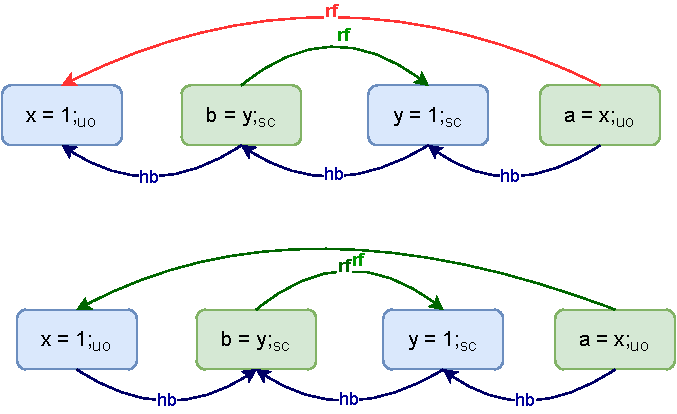
\includegraphics[scale=0.7]{5.InstructionReordering/0.Intro/ReorderingExample2(b).pdf}
            \caption{The set of partial order relations justifying the observable behavior in question for both the candidates in Figure~\ref{reord:example2(a)}.} 
            \label{reord:example2(b)}
        \end{figure}

        The above two examples show that we have to be careful while reordering two events in the same thread. 
        By example analysis, for each observable behavior, one must check all possible candidate executions and assert whether such an observable is possible or not. 
        This method of checking validity of reordering will scale exponentially as the program size increases. 
        It may also be the case that the compiler may not have information on which exact events would be executed in other threads to assert such reordering is valid. 

    
    
    
    
    


%The end ? ------------------------------------------------------------------------------------------------------------------------------    
    
\end{document}
